\section{分配格}
一般地,偏序格不满足分配律.

例如,由\hyperref[figure:格论.偏序集2]{钻石格的哈斯图}可知\begin{gather*}
	a \cdot (b + c) = a \cdot 1 = a, \\
	(a \cdot b) + (a \cdot c) = 0 + 0 = 0,
\end{gather*}
从而\(a \cdot (b + c) \neq (a \cdot b) + (a \cdot c)\),
即钻石格的\(\cdot\)运算对\(+\)运算不可分配.

\begin{figure}[hbt]
%@see: 《离散数学》(邓辉文) P155 图5-3(a)
	\centering
	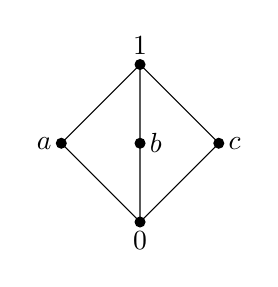
\begin{tikzpicture}
		\fill(0,0)circle(2pt)node[above]{$1$};
		\fill(1,-1)circle(2pt)node[right]{$c$};
		\fill(0,-1)circle(2pt)node[right]{$b$};
		\fill(-1,-1)circle(2pt)node[left]{$a$};
		\fill(0,-2)circle(2pt)node[below]{$0$};
		\draw(0,0)--(1,-1)--(0,-2)--(0,0)--(-1,-1)--(0,-2);
	\end{tikzpicture}
	\caption{钻石格的哈斯图}
	\label{figure:格论.偏序集2}
\end{figure}

类似地,由\hyperref[figure:格论.偏序集3]{五角格的哈斯图}可知,
五角格的\(\cdot\)运算对\(+\)运算不可分配.

\begin{figure}[hbt]
%@see: 《离散数学》(邓辉文) P155 图5-3(b)
	\centering
	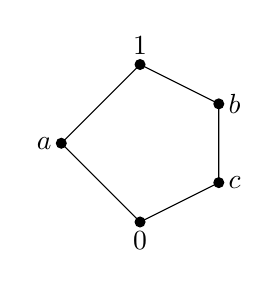
\begin{tikzpicture}
		\fill(0,0)circle(2pt)node[above]{$1$};
		\fill(1,-.5)circle(2pt)node[right]{$b$};
		\fill(1,-1.5)circle(2pt)node[right]{$c$};
		\fill(0,-2)circle(2pt)node[below]{$0$};
		\fill(-1,-1)circle(2pt)node[left]{$a$};
		\draw(0,0)--(1,-.5)--(1,-1.5)--(0,-2)--(-1,-1)--(0,0);
	\end{tikzpicture}
	\caption{五角格的哈斯图}
	\label{figure:格论.偏序集3}
\end{figure}

\begin{definition}
%@see: 《离散数学》(邓辉文) P158 定义5-23
设\(\opair{L,\leq}\)是偏序格.
若\(L\)的\(\cdot\)运算对\(+\)运算可分配,
或\(L\)的\(+\)运算对\(\cdot\)运算可分配,
则称“\(\opair{L,\leq}\)是\DefineConcept{分配格}(distributive lattice)”.
\end{definition}

\begin{example}
%@see: 《离散数学》(邓辉文) P158 例5-32
设\(X\)是非空集合.
证明:\(\opair{\Powerset X,\subseteq}\)是分配格.
%TODO proof
\end{example}

\begin{example}
设\(F\)是全体合式公式,\(\implies\)是逻辑蕴含关系.
证明:\(\opair{F,\implies}\)是分配格.
%TODO proof
\end{example}
